\documentclass{article}
\usepackage[utf8]{inputenc}



\usepackage{natbib}
\usepackage{graphicx}


\begin{titlepage}

\newcommand{\HRule}{\rule{\linewidth}{0.5mm}} 

 

\center


\textsc{\Large SOEN6011(Deliverable 3)}\\[0.5cm] 
\url{https://github.com/vik-sandhu/soen$\_$6011  }\\[0.5cm] 


\HRule \\[0.4cm]
{ \huge \bfseries Source Code Review}\\[0.4cm] 
\HRule \\[1.5cm]
 


\begin{minipage}{0.4\textwidth}
\begin{flushleft} \large
\emph{Author:}\\
VIKRAMJIT \textsc{SINGH} 
\end{flushleft}
\end{minipage}
~
\begin{minipage}{0.4\textwidth}
\begin{flushright} \large
\emph{Student ID:} \\
40075774 \textsc{ } 
\end{flushright}
\end{minipage}\\[2cm]



{\large \today}\\[2cm] 


\includegraphics[width=8cm,height=4cm,keepaspectratio]{logo.jpg}\\[1cm] 

\vfill 

\end{titlepage}


\pagebreak
\tableofcontents
\pagebreak

\begin{document}



\pagebreak
\chapter{Problem 5}
\section{Source Code Review $\sinh(x)$}
 According to the professor's instructions, for problem 7, F2 reviews F3. So, for problem 5, I reviewed source code of $\sinh(x)$. I reviewed this source code both manually and automatically. 
 \subsection{Automatic source code review}
 For Automated source code review, I used PMD (Programming Mistake Detector), which is a open source static source code analyzer that reports on issues found within application code. Issues announced by PMD are about inefficient code, or terrible programming propensities, which can decrease the exhibition and viability of the program.
 \begin{flushleft}
 I used PMD plugin in Eclipse IDE to review the source code. The report (text file) generated by PMD is attached within this  deliverable(D3) under the name of pmd-report. The violations in the source code are listed in this report.
 The images below shows various violations shown on console.
 \end{flushleft}
 
 \begin{figure}[h!]
  \centering
 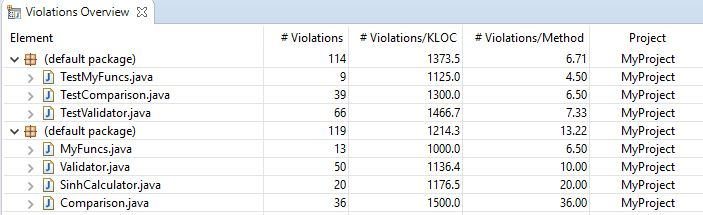
\includegraphics[width=16cm,height=30cm,keepaspectratio]{pmd1.jpg}\\[1cm] 
  \caption{PMD console output}
\end{figure}

\begin{figure}[h!]
  \centering
 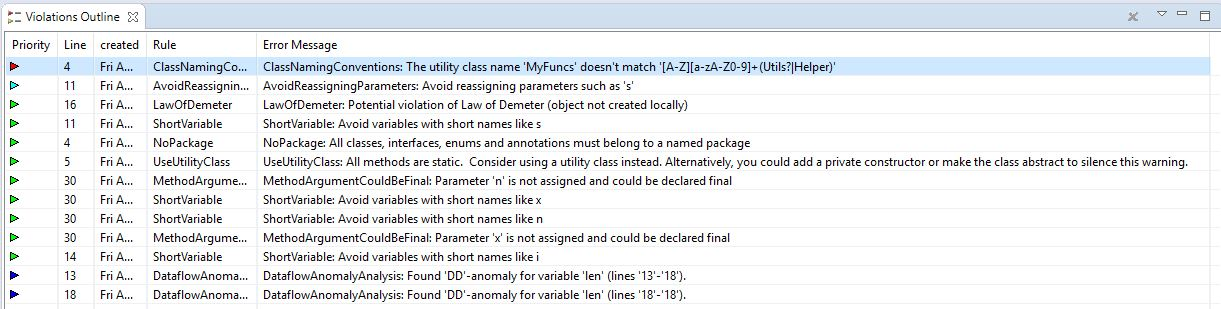
\includegraphics[width=16cm,height=30cm,keepaspectratio]{pmd2.jpg}\\[1cm] 
  \caption{PMD console output}
\end{figure}

\begin{flushleft}
In the Figure 2
\begin{itemize}
    \item Red arrow depicts Blocker Violations.
    \item Turquoise arrow depicts Critical Violations.
    \item Green arrow depicts  Urgent Violations.
    \item Pink arrow depicts Important Violations.
    \item Blue arrow depicts Warning Violations
\end{itemize}
\end{flushleft}
\subsection{Manual Source Code Review}
After comprehending the entire source code, I came across various flaws in this source code which are listed below.
 \begin{itemize}
     \item Our team decided to abide by Google Java Style Guide. But coding standards are not followed throughout the project.
     \item Incorrect identation throughout the project.
     \item Class Naming Conventions are also not followed, in the whole project.
     \item In the whole project, the variables names used are very small like i,x. Instead meaning full variables names should be used.
     \item The class Comparison has very high complexity. Complexity can be reduced using efficient loops or a better approach.
     \item Only variables that are final can contain underscore in their names, but in class Comparison contains many variables that are not final and contain underscore in their names. For example: value\_positive, abs\_x etc.
     \item Avoid using literals in conditional statements.
     \item Value of some local variables like len, count is never used.
     \item Resource Leak: Scanner sc is never closed.
     \item Public methods and constructors comments are missing.
     \item Some comments are too long.
     
 \end{itemize}

 


\pagebreak
\chapter{Problem 7}
\section{Testing Review $\log_{b} (x)$}
$tan(x)$ (F2) is the function assigned to me. According to the professor's instructions, for problem 7, F2 reviews F4. So, for problem 7, I tested $\log_{b} (x)$.
\begin{flushleft}
 I used JUnit to compute the result of the test cases. All the five test cases passed and it took just 0.031 seconds to all run the test cases which proves system efficiency. These test cases covered mostly all the functionality.The programmer had a clear and user friendly GUI.
 \end{flushleft}

\begin{figure}[h!]
  \centering
  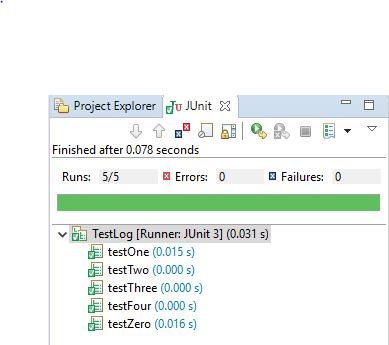
\includegraphics[width=20cm,height=10cm,keepaspectratio]{report.jpg}\\[1cm] 
  \caption{Test Output}
\end{figure}

 During testing, I also found certain inconsistencies which are listed below.

\begin{itemize}
   \item Missing Javadoc comments.
   \item Incorrect identation.
   \item Some lines contained tab character. 
   \item Should have added more test cases to show what happens when negative value is entered by the user.
   \item Though the test case testOne is passed in JUnit, but in this test case the output given by the function is wrong. Value of $\log_{1} (1)$ is undefined, but according to this program output is 0, which according to me is a major discrepancy.
   \item According to FR2, x can never be 0. But in test case testZero, user input x as 0 and still gets output from the program. In this case, output should be Math Error.
\end{itemize}



 
 

\begin{thebibliography}{}

\bibitem{link}
{https://en.wikipedia.org/wiki/PMD}
\bibitem{link}
{https://en.wikipedia.org/wiki/JUnit}

\end{thebibliography}
\end{document}
